\chapter{Plan for Developing the Solution}

In this section an overview of the design and architecture of the project is provided. Then, choices on the technology such as programming languages and databases are explained. Finally, a project plan is laid out.



\section{Design \& Architecture}

The architecture of this project is designed to meet the requirements discussed in section \ref{problem}. First, a bird's eye view is given on where this recommender framework fits into existing systems. Then, the internal architecture of the framework is explained.

\subsection{Service-Oriented Architecture (SOA)}
\label{sol-design-soa}

\begin{figure}[ht]
    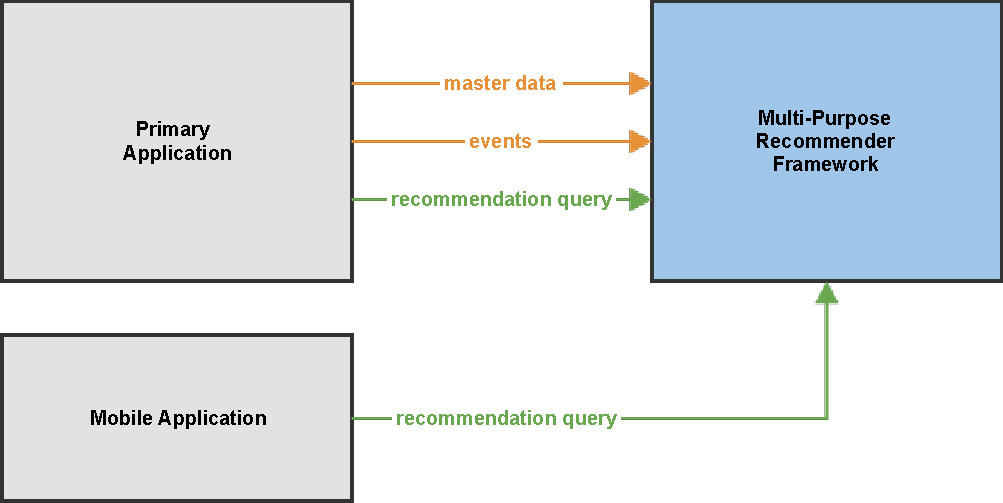
\includegraphics[width=0.7\textwidth,center]{solution/soa/soa.pdf}
    \caption[Service-Oriented Architecture (SOA)]{Service-Oriented Architecture (SOA). Orange arrows (\emph{master data} and \emph{event}) are \emph{notifications} whereas green arrows (\emph{recommendation query}) are \emph{queries} and expect a result.}
    \label{fig:soa}
\end{figure}

A \emph{service-oriented architecture (SOA)} is a software design pattern which is most suitable to meet the \emph{abstraction} requirement discussed in section \ref{problem-abstraction}. \emph{SOA} suggests to express features as services. This is true for features which are going to be available to other systems. Internal features are never to be exposed and allowed to be services. A \emph{service consumer} is a system using the service. \cite{erl08} identifies eight principles of \emph{SOA} of which I will elaborate four:

\begin{description}
    \item[Standardised service contracts] is an expression of the service's purpose, capabilities and requirements -- such as mandatory parameters and data types. As long as the requirements are satisfied, the service agrees to fulfill its purpose.
    \item[Service loose coupling] makes sure that services have as few dependancies as possible.
    \item[Service abstraction] ensure that as much information as possible hidden and none except those described in the service contract are exposed.
    \item[Service reusability] assure that services are designed to be reused.
\end{description}

In figure \ref{fig:soa} a possible architecture of the project is shown. The framework is designed to serve more than one application or system component. The services accept requests from any source as long as they authorise with an access key. In the mentioned figure services are divided in two types -- \emph{notification} and \emph{query}. A \emph{notification} is a message relevant to the recommender framework and is simply acknowledged as received. A \emph{query} on the other hand expects a result. The framework will define three services:

\begin{description}
    \item[Master Data] enables service consumers to create, update or delete a data node in the framework. An identifier and type are mandatory fields. The service consumer is allowed to send any further features of the node which it thinks is relevant to the framework.
    \item[Event] accepts notifications about interactions or preferences between two or more nodes such as \emph{'X purchased Y and Z'}. The payload -- content of the message -- may contain a \emph{weight} which is a numeric value. It is useful for e.g. \emph{'X rated Y with 10'}.
    \item[Recommendation Query] requests recommendations for a specific \emph{recommendation model}. The recommendation model identifier is mandatory. A node identifier and type are only mandatory if the model excepts it. This is the only service which expects a result.
\end{description}

The recommendation framework only expects incoming requests (\emph{push strategy}) and has no outgoing communication at all.

\subsection{Multi-Layered Architecture}
\label{sol-design-layer}

\begin{figure}[ht]
    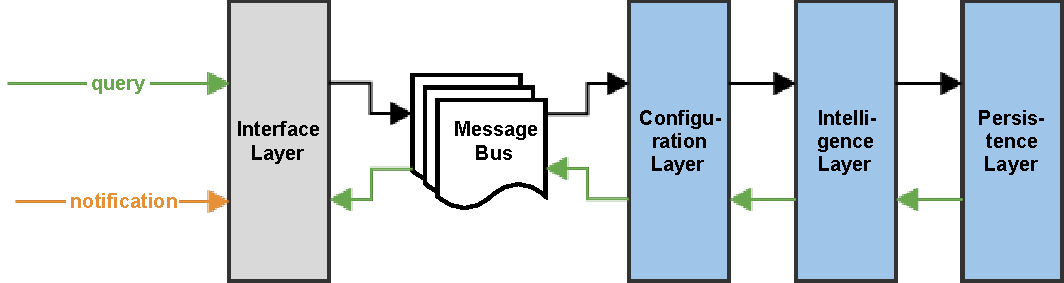
\includegraphics[width=\textwidth,center]{solution/layers/layers.pdf}
    \caption{Multi-Layered Architecture}
    \label{fig:layers}
\end{figure}

A multi-layered architecture is a software design pattern for software programs which suggests separating functionality in responsibility layers. This is popular way of abstracting functionality within a system.

Strictly speaking, the framework is divided into two subsystems: the \emph{application programming interface (API)} and \emph{recommender ecosystem}. These subsystems are connected via message bus. The motivation of this differentiation is of a technical rather than logical nature. The subsystems have different kind of technical requirements and this division allows me to use respectively the most appropriate technology. Another side effect is that a message bus allows me to group and prioritise messages.

\subsubsection{Interface Layer}
\label{sol-design-layer-interface}

The interface layer is where services expose themselves to service consumers which are those components sending requests to this layer. From a technical point of view this layer is implemented as an \emph{application programming interface (API)} over the \emph{hypertext transfer protocol (HTTP)} which is the foundation of data communication in the world wide web. The \emph{API} adopts the \emph{representational state transfer (REST)} style. An \emph{API} which uses \emph{REST} is called \emph{RESTful}. 

\emph{REST} makes use of \emph{uniform resource locators (URLs)} and \emph{HTTP vocabularies} which is of importance for this project. The \emph{URL} provides a way to locate a resource. The \emph{HTTP vocabulary} defines amongst others \emph{GET}, \emph{POST} and \emph{DELETE}. Combined a \emph{RESTful API} enables the access and modification of resources. E.g. to submit an event a \emph{POST} request to \emph{/events} is necessary. To delete a node with the identifier \emph{120} a \emph{DELETE} request to \emph{/nodes/120} is sufficient, whereas a \emph{GET} request to \emph{/recommendations/topseller} would return all recommendations for a recommendation model called \emph{topseller}. By using low-level \emph{HTTP} vocabulary the \emph{API} requires less documentation and explanation \cite{fielding00}.

This layer acts as \emph{service broker} and \emph{security agent}. Latter is ensured by verifying the presence and correctness of an access key which is a random text. As a \emph{service broker} this layer validates the payload against mandatory fields and data types. Then, it offloads the message and submits it into the message bus for further processing. If the message is of the type \emph{notification} it acknowledges the request. If the message type is a \emph{query}, then it waits for a response from the message bus and returns that.

\subsubsection{Configuration Layer}
\label{sol-design-layer-config}

This layer is the heart of this project and targets to satisfy the multi-purpose and interoperability requirement (as defined in \ref{problem-multipurpose}). The motivation behind this layer is to set up a recommender system by configuration only. The configuration layer consists of two fundamental ideas: the \emph{recommendation model} and \emph{event}.

A \emph{recommendation model} is an instruction to the recommender on how to compute recommendations. In the model configuration identifier, recommender type and optional parameter are specified.

As mentioned in section \ref{sol-design-soa}, an event is the information about an interaction between two or more nodes such as \emph{'X purchased Y and Z'}. The event subsystem provides a mechanism to allow recommendation models to listen to events. When an event message is received, the subsystem will inform listeners. This way recommendation models receive new data and one event can be used by more than one recommendation model. In a traditional architecture the application would need to update every single recommender system. However the event subsystem makes redundant API calls obsolete as only one message is sufficient. Figure \ref{lst:recomodel-config} shows an example configuration.

\begin{figure}[ht]
    \xmlfile{listings/solution/recommendation.xml}
    \caption{Recommendation Model Configuration}
    \label{lst:recomodel-config}
\end{figure}

\subsubsection{Recommendation Layer}
\label{sol-design-layer-reco}

In the \emph{recommendation layer} holds the actual recommenders which are associated to recommendation models by the configuration layer. The recommender are going to be unaware of the nature of the data. In the contrary it will work based on the parameters fed by the configuration layer. Then, the algorithm will build its algorithm-specific query and use the persistance layer to fetch data and eventually return recommendations.

A distinctive feature of this project will be the recommender plug-in subsystem. All recommenders will be designed as extensions.

\subsubsection{Persistance Layer}

This layer provides database abstraction components which will then allow any recommender system to access any of the supported storage systems.



\section{Technological Choices}

In this section I will discuss my choices in technology I want to use in this project.

\subsection{Application Programming Interface (API)}

The \emph{API} is the interface layer in this project and defines almost none business logic. In that sense it is important to use a lightweight, thin solution. As discussed in \ref{sol-design-layer-config} I will use a \emph{RESTful} approach for the \emph{API}.

The \emph{API} will be built on the \emph{node.js} platform which makes use of \emph{Google Chrome}'s fast \emph{V8 JavaScript engine}. The \emph{API} will further use \emph{express} -- a web application framework for \emph{node.js}. \emph{express} is ideal for \emph{RESTful APIs} as it uses the \emph{HTTP} vocabulary as well. Figure \ref{lst:expressjs} illustrates a sample implementation of `\emph{GET} request to \emph{/recommendations/topseller}' mentioned in \ref{sol-design-layer-interface}. As visible in the figure the footprint of the implementation is very thin. As the \emph{API} has a specific format in \emph{express}, it is able to automatically generate \emph{API} documentation.

\begin{figure}[ht]
    \jsfile{listings/solution/express.js}
    \caption{Sample API for recommendations in \emph{express}}
    \label{lst:expressjs}
\end{figure}

The message format will be in \emph{JavaScript Object Notation (JSON)} - a thinner alternative to \emph{extensible markup language (XML)}.




\subsection{Message Bus}

The concept of the message bus was introduced in section \ref{sol-design-layer}. The main requirement is that it implements the \emph{advanced message queuing protocol (AMQP)} -- an open standard which defines a minimum set of features in message buses. A popular, highly reliable message bus software which supports \emph{AMQP} is \emph{RabbitMQ}. It also provides a \emph{graphical user interface (GUI)} giving information about the current message flow. I have worked with \emph{RabbitMQ} in the past.

\subsection{Recommender Ecosystem}

This subsystem contains configuration, intelligence and persistence layers. It needs to be performant due to the implementation of recommenders which can require a lot of computing resources. In that sense dynamic scripting languages such as \emph{hypertext preprocessor (PHP)} or \emph{Python} are not my first choice. In fact a statically-typed, compiled language with concurrency capabilities is needed.

My preferred candidate for this is \emph{Go} -- a language developed by \emph{Google} as an alternative to overcome limitations of the programming language \emph{C++}. The result is a language which is intendedly not adopting all patterns found in many programming languages such as overloading and pointers. The language aims to be simple, safe and free of misinterpretations by the compiler. It supports multithreading, CPU paralleling as well as asynchrony. Finally, it has a modern package management system which allows retrieving packages from the internet.

\subsubsection{Database Software}

The recommender ecosystem requires a powerful yet flexible database software. As pointed out in section \ref{sol-design-soa} a master data can have an arbitrary number of additional fields. To fulfill the \emph{ease of integration} requirement a schema management solution is not desired. Schema-less databases -- also known as \emph{NoSQL} -- might be of interest. \emph{NoSQL} databases are usually non-relational as well. However recommendations are very intensive in terms of relations (e.g. \emph{`X rated Y'}).

A potential solution are graph databases which understand \emph{nodes} and \emph{edges} -- relations to nodes. A \emph{property} can be attached to \emph{nodes} as well as \emph{edges}. Latter is useful for weighted relations such as \emph{`X rated Y with 10'}. Figure \ref{fig:graph} shows a sample graph. Graph databases have further advantages especially in querying distant \emph{nodes} via other \emph{nodes}. With regard to figure \ref{fig:graph}, an example query could be to fetch all groups people, who Alice knows, are members of.

\begin{figure}[ht]
    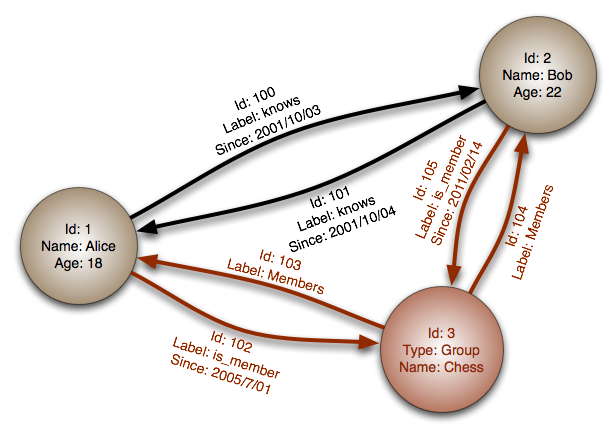
\includegraphics[width=0.7\textwidth,center]{solution/tech/graph.png}
    \caption[Simple Graph in a Graph Database]{Simple Graph in a Graph Database. Source: Creative Commons.}
    \label{fig:graph}
\end{figure}

\subsection{Others}

A \emph{version control management (VCS)} namely \emph{git} will be used throughout the project. \emph{Git} is a distributed \emph{VCS} which is amongst others faster and more flexible than other \emph{VCS} such as \emph{Subversion}. The \emph{git} repository -- and therefore the source code -- will be hosted on \emph{BitBucket} to have a backup of the project anytime.

For server health and performance monitoring I will use the \emph{software as a service (SAAS)} solution \emph{NewRelic}. It also allows to analyse specific low performing or faulty requests. This will be very useful during testing and evaluation of the solution.

\begin{figure}[ht]
    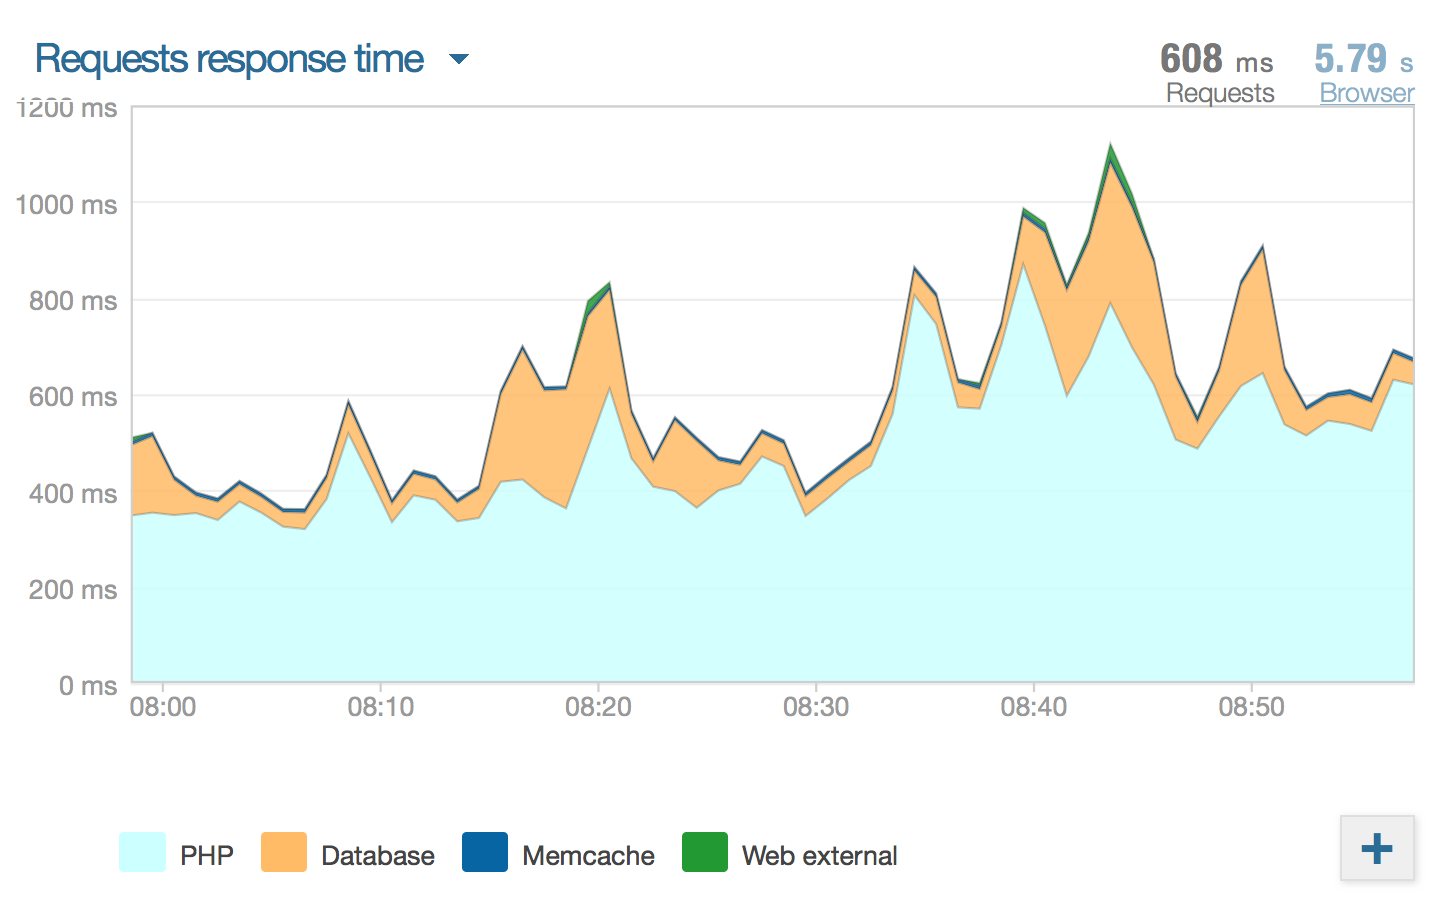
\includegraphics[width=0.7\textwidth,center]{solution/tech/newrelic.png}
    \caption{Monitoring with NewRelic}
    \label{fig:newrelic}
\end{figure}

Finally, a virtualisation solution called \emph{VirtualBox} will be used to set up all technical and vendor requirements within a virtual machine. This prevents conflicts with dependencies on the workstation especially if versions differ. When submitting the project the virtual machine will be packaged to provide a seamless demo setup for examination.



\section{Demo}

\begin{figure}[!ht]
    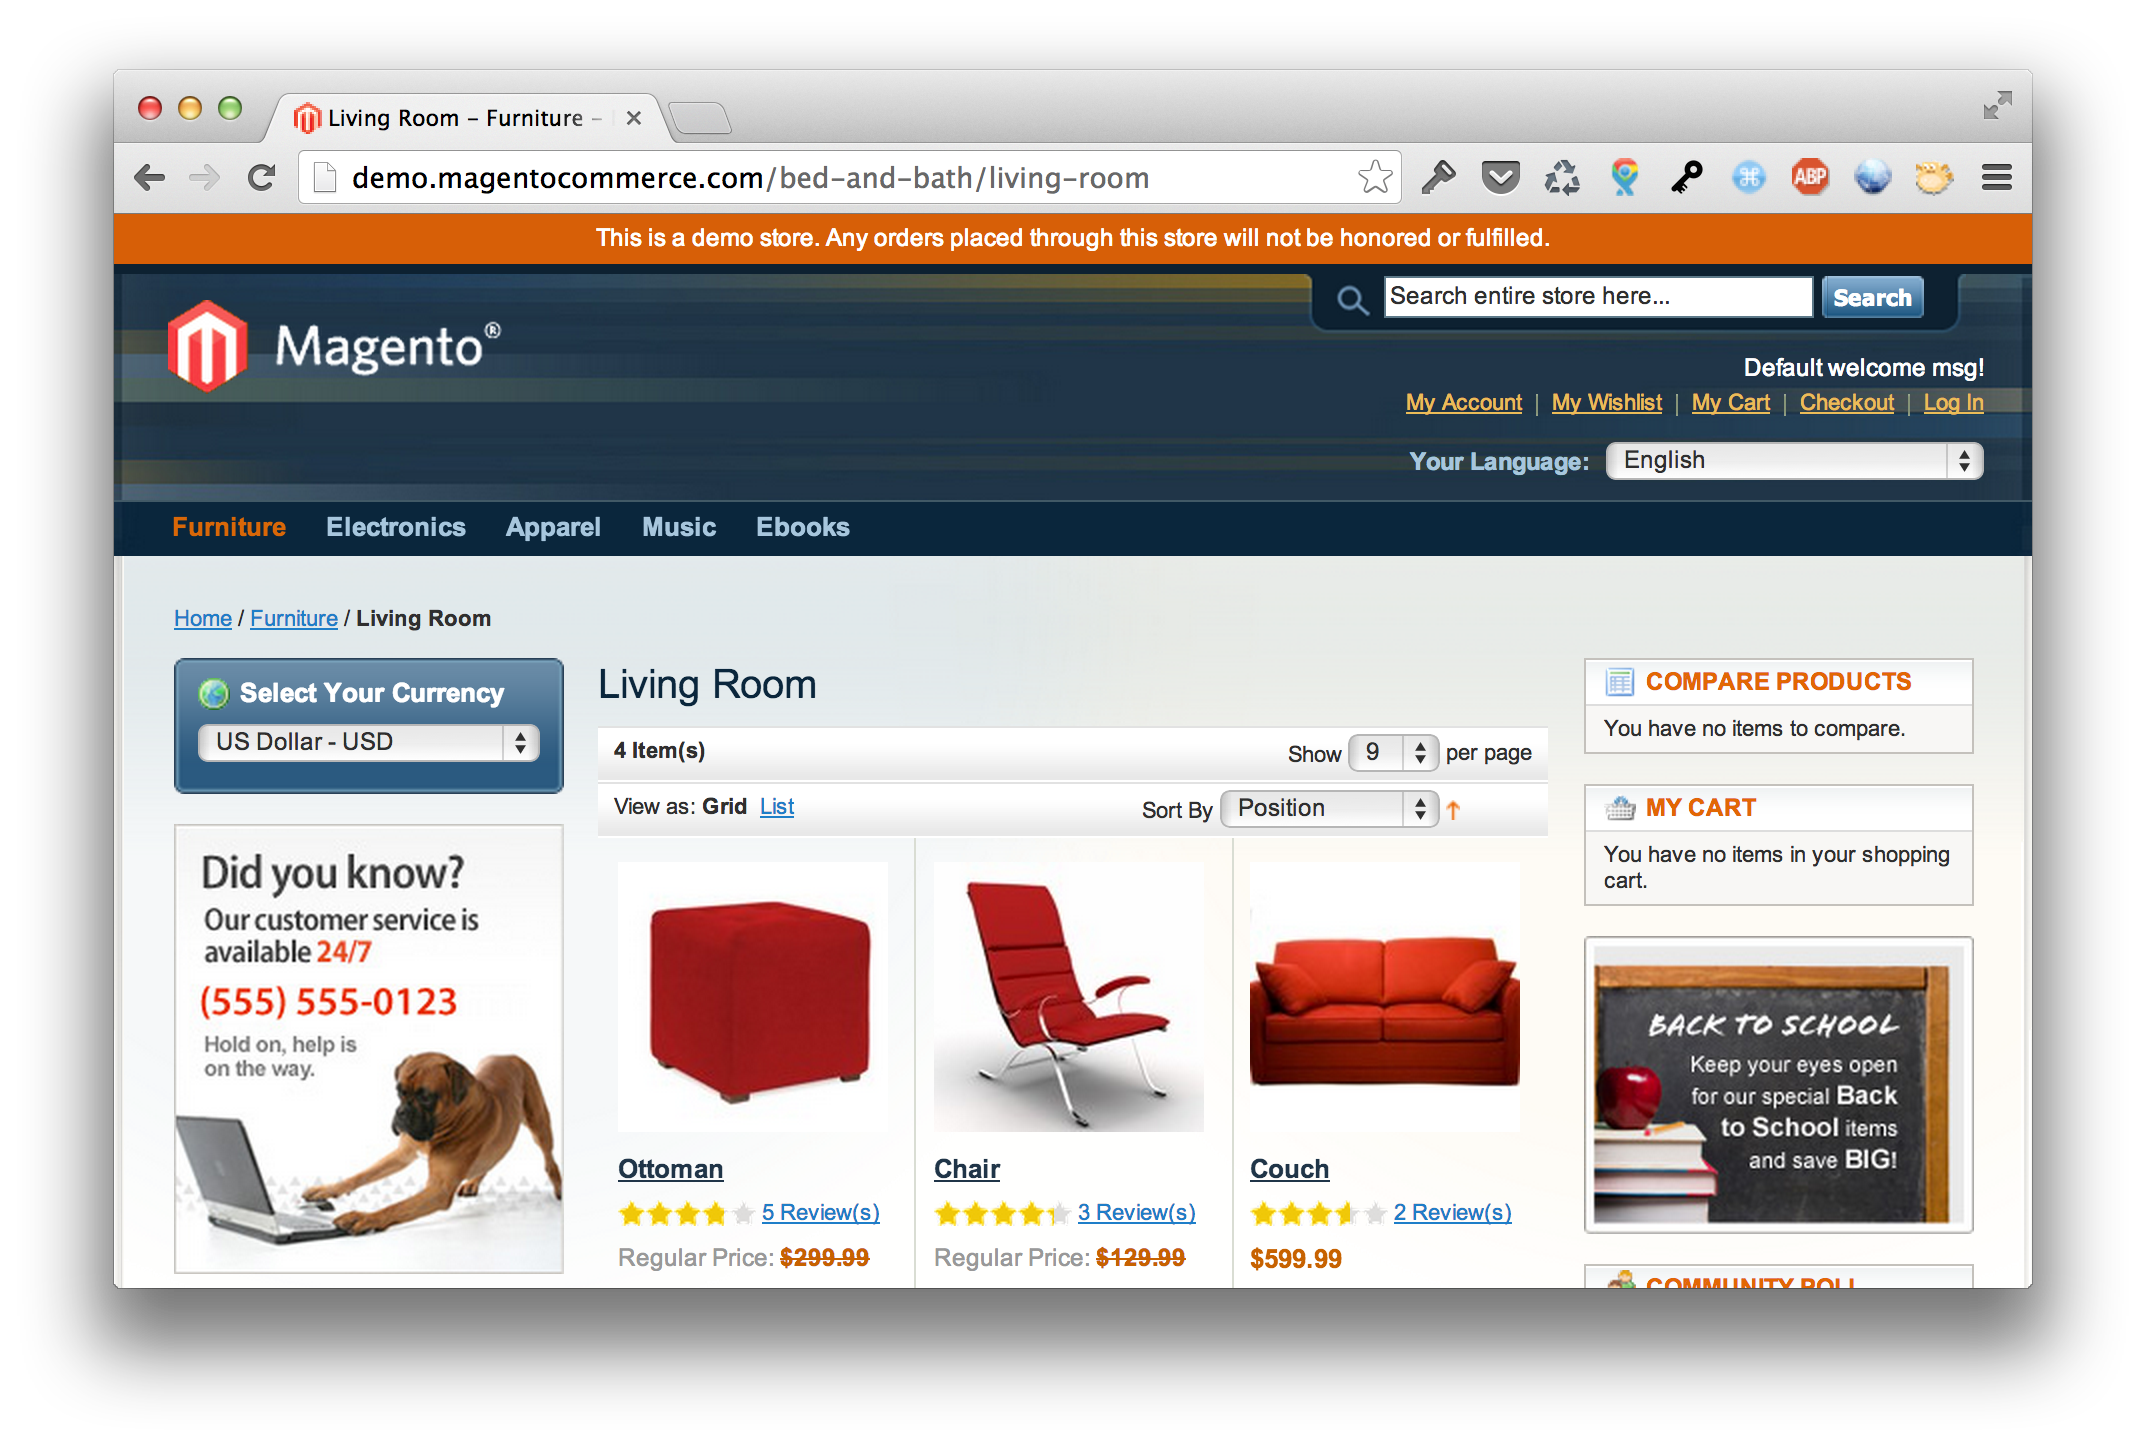
\includegraphics[width=\textwidth,center]{solution/tech/magento.png}
    \caption{Open-Source Ecommerce Web Application \emph{Magento}}
    \label{fig:magento}
\end{figure}

The proposed architecture primarily deals with internals. Although it can be tested by simulating \emph{API} calls, it is not very visible and tangible. Therefore the solution will be demonstrated on a platform which reflects a real-life use case. As seen in the background research most applications using recommender systems are e-commerce websites. 

It is hence not surprising that the demo will be as well an e-commerce website which will be based on the open source e-commerce web application \emph{Magento} -- strictly speaking the free community edition. Having used \emph{Magento} professionally I am comfortable extending it for my testing purposes. The product database will be loaded with ca. hundred thousand individual products which allows us to evaluate basic scalability and performance testing.



\section{Project Plan}

This section provides a work schedule to complete the project as well as a fallback plan in case of unexpected or time-related circumstances.

\subsection{Schedule}

The project will be split into two broad phases: \emph{implementation} and \emph{evaluation}. The implementation phase is from 5th May to 10th August 2014, then the evaluation phase is until 15th September 2014. As the project has significant implementation work to be done, this strict division makes sure that enough time is left for the evaluation phase.

The schedule in figure \ref{fig:schedule} is divided into bi-weekly time frames in which one or more tasks are to be delivered. 

\renewcommand{\arraystretch}{1.5}
\begin{figure}[ht]
    \small
    \begin{tabularx}{\textwidth}{
        !{\vrule width 1pt} c !{\vrule width 1pt} c !{\vrule width 1pt} X !{\vrule width 1pt}
    }
        \noalign{\hrule height 1pt}

        & \textbf{Time Frame} & \textbf{Tasks}\\

        \noalign{\hrule height 1pt}

        & 5th - 18th May & 
        Set up virtual machine as well as Magento.\newline
        Implement interface layer.\newline
        Implement publishing to message bus.
        \\\cline{2-3}

        \multirow{5}{*}{\begin{sideways}\textbf{Implementation}\end{sideways}} & 19th May - 1st June & Implement master data service.\\\hhline{|~|-|-|}

        & \cellcolor{codebg}2nd - 15th June & \cellcolor{codebg}Exam Break\\\cline{2-3}

        & 16th - 29th June & Implement event service.\\\cline{2-3}

        & 30th June - 13th July & Implement plug-in system for recommender techniques.\\\cline{2-3}

        & 14th - 27th July & Implement recommendation model service.\\\cline{2-3}

        & 28th July - 10th August & Implement several recommender techniques.\\

        \noalign{\hrule height 1pt}

        \multirow{6}{*}{\begin{sideways}\textbf{Evaluation}\end{sideways}} & 11th - 24th August & 
        Evaluation of architecture and recommendation quality.\newline
        Structure report.
        \\\cline{2-3}
        
        & 25th August - 7th September & Write chapters of the report related to implementation and architecture.\\\cline{2-3}

        & 8th - 15th September & Write remaining chapters of report and finalize.\newline
        Write documentation.\\

        \noalign{\hrule height 1pt}
    \end{tabularx}
    \caption{Project Schedule}
    \label{fig:schedule}
\end{figure}

\subsection{Fallback Plan}

In this section alternative paths are defined in case of delays due to underestimated work or other external circumstances.

The software architecture is the critical path of the project. Little is gained when layers or distinctive features are missing. Therefore I will focus on delivering them. In case of delays it is possible to decrease the number of different techniques and recommendation uses cases. In the worst case scenario, a the requirements of recommendations can be kept low so that I can use simpler recommender systems.

\emph{Go} and \emph{Neo4j} are yet unfamiliar to me. In case of problems, they can be replaced by simpler or more familiar choices. \emph{Go} itself could be replaced by \emph{PHP} or \emph{Python}. Instead of \emph{Neo4j} the key-value store \emph{Redis} may be a simple alternative.